\documentclass[a4paper]{report}

\makeindex
\usepackage{url}
\usepackage[T1]{fontenc}
\usepackage[colorlinks=true,urlcolor=blue,linkcolor=blue,breaklinks=true]{hyperref}
\usepackage[utf8]{inputenc}
\usepackage{graphicx}
\usepackage{geometry}
\usepackage[explicit]{titlesec}
\usepackage[outputdir=out]{minted}
\usepackage{xcolor}
\usepackage{caption}
\usepackage{subcaption}

\geometry{a4paper, margin=2.54cm}

\usepackage{xepersian}
\settextfont{IRNazanin}[
	Extension=.ttf,
	BoldFont=*Bold,
	ItalicFont=*Italic,
	BoldItalicFont=*Bold,
	Path=fonts/
]

\def\addbibtoc{
	\addcontentsline{toc}{section}{\numberline{\mbox{}}\relax\bibname}
}
\setcounter{page}{1}

\newcommand{\subfigr}[2]{
	\begin{subfigure}{0.5\textwidth}
		\includegraphics[width=\textwidth]{#1}
		\caption*{#2}
	\end{subfigure}
}

\begin{document}
\begin{titlepage}
\centering
{
\includegraphics[width=3cm]{assets/logo.png}}\\[0.5cm]
گروه کامپیوتر دانشگاه آزاد مشهد\\[1cm]
{\LARGE \textbf{گزارش عملکرد پروژه رسم و محاسبه سری فوریه}}\\[1cm]
با نظارت: استاد داوود علی‌اکبری\\[0.5cm]
دانشجو: سید علیرضا ارزه گر\\[0.5cm]
\today\\[1cm]
\end{titlepage}

\cleardoublepage

\tableofcontents
\newpage

\section{مقدمه}

این گزارش به بررسی عملکرد پروژه ترسیم و محاسبه سری فوریه برای درس ریاضیات مهندسی دانشگاه آزاد
با نظارت استاد داوود علی‌اکبری می‌پردازد. در ابتدا می‌توانید پروژه را از مخزن گیتهاب دریافت نمیایید.
\LTRfootnote{https://github.com/alirezaarzehgar/fouriersolver}
این گزارش برای ورژن \lr{v1.1.0} این پروژه را شامل می‌شود و الزاما برای نسخه‌های آینده پروژه صادق نمی‌باشد.
لزا توجه داشته باشید. لطفا از درست بودن تگ و ورژن این پروژه اطمینان حاصل کنید.

\subsection{هدف کلی پروژه}

این پروژه قصد دارد با دریافت $f(x)$ از کاربر و بازه $x$ یک سری را به‌واسطه بسط فوریه ترسیم کند.
اولین چالش دریافت ورودی‌های مناسب از کاربر بوده و سپس باید از بسط فوریه برای نمایش این سری استفاده کرد.
ابتدا به ساکن بر اساس مفاهیم فوریه، این پروژه می‌تواند تمام ضرایب $a_n$ و $b_n$ را محاسبه کند. تمام پارامترهای
لازم باید قابل تنظیم باشند. من جمله مقدار $n$، دقت محاسبه انتگرال، تنظیمات مربوط به رابط‌هایی مانند
\lr{gnuplot, desmos, geogebra}
و غیره. پس کلیت هدف پروژه دریافت یک سری ورودی، پردازش آن و ارائه خروجی مناسب بر اساس آپشن‌های کاربر می‌باشد.

\section{معماری پروژه}
\subsection{محیط توسعه}
این پروژه بر روی سیستم‌عامل آرچ لینوکس
\LTRfootnote{Archlinux}
توسعه و تست شده است. انتظار می‌رود پروژه برای تمامی سیستم‌عامل‌های \lr{GNU/Linux} قابل استفاده باشد و حداکثر
با اندکی تغییر برای باقی سیستم‌عامل‌های خانواده یونیکس مانند \lr{Mac OS} پورت شود.
{\large توجه:}
این پروژه برای حل چالش‌های خود از مفاهیم یونیکسی و استانداردهای آن استفاده کرده است و قابل اجرا در ویندوز نخواهد بود.
برای اجرا در ویندوز نیاز به پورت کردن وجود دارد.

\subsubsection{چرا یونیکس؟}
ممکن است این سوال ایجاد بشود که چرا محیط توسعه و پلتفرم هدف این پروژه مایکروسافت ویندوز نیست.
در ابتدا به ساکن باید اشاره شود که انتخاب یونیکس تا حد زیادی بر سلیقه توسعه دهنده این پروژه استوار است.
توسعه دهنده ای که سالها با سیستم‌های یونیکسی و لینوکس تعامل داشته و درحال حاضر نیز ویندوز در دسترس ندارد
نباید انتخاب بهتری از یک سیستم‌عامل یونیکسی داشته باشد. هرچند نوشتن برنامه‌های سازگار با لینوکس مزایای بیشتری
تا صرف سلیقه دارد.

دیزاین بر اساس استانداردهای ویندوز، طراحی پروژه را به یک پلتفرم محدود خواهد کرد. در مقابل طراحی سیستم بر اساس
استاندارد هایی مانند \lr{POSIX}
\LTRfootnote{Portable Operating System Interface}
و سازگاری با یونیکس، اپلیکیشن را برای خانواده ای از سیستم‌عامل‌ها قابل اجرا می‌سازد.

جامعه هدف این پروژه استاد محترم درس ریاضیات مهندسی، استاد داوود علی‌اکبری و جامعه متن‌باز
\LTRfootnote{Open Source}
می‌باشد. از دیر باز محیط‌های آکادمیک حامی پروژه‌های متن باز بوده اند و حتی خیلی از پروژه‌های متن باز دنیا زیر نظر دانشگاه‌های
برتر دنیا توسعه داده شده اند. برای مثال به سیستم‌عامل بی‌اس‌دی در دانشگاه برکلی، پروژه اوپن سی‌وی در دانشگاه میشیگان، 
مفسر متن‌باز متلب به نام گنو اوکتاو در دانشگاه تگزاس اشاره کرد. این پروژه نیز قصد دارد با استانداردهای جهانی و علمی دنیای
کامپیوتر سازگار باشد و حدالامکان طراحی صحیحی از نظر توسعه نرم‌افزار داشته باشد. درواقع خاطب هدف این پروژه مانند پروژه‌های
مذکور خواهد بود.

\subsection{چه استانداردهایی در این پروژه رعایت شده است؟}
پروژه‌های مختلف از قراردادهای
\LTRfootnote{convention}
مختلفی استفاده می‌کنند. یکی از این قراردادها استایل کد پروژه می‌باشد. این پروژه از استایل کد لینوکس
\LTRfootnote{\url{https://www.kernel.org/doc/html/v4.10/process/coding-style.html}}
استفاده می‌کند و بر این اساس توسعه و نگهداری می‌شود.

سیستم ساخت
\LTRfootnote{Build System}
پروژه با استفاده از \lr{GNU Make} طراحی شده است و همانطور که اشاره شد از استانداردهای \lr{POSIX} پیروی می‌کند.

سادگی و طراحی صحیح به همراه کامل بودن اصلی ترین هدف این پروژه می‌باشد.

این پروژه تحت مجوز \lr{GPL}
\LTRfootnote{GNU General Public License}
توسعه یافته است و می‌توانید به‌صورت آزاد آن را توزیع کرده و توسعه دهید.

این پروژه کاملا سازگار برای محیط‌های خط فرمان می‌باشد.

\subsection{طریقه کامپایل و نصب اپلیکیشن}
برای دانلود و نصب این اپلیکیشن ابتدا از نصب بودن نیازمندی‌های آن مطلع باشید. یونیکس شما باید پیش از اجرای برنامه
کامپایلر سی
\LTRfootnote{GCC(GNU C Compiler)}، 
بسته \lr{gnuplot}، و همینطور \lr{texlive} را برای تولید مستندات داشته باشد.

پس از نصب نیازمندی‌ها می‌توانید با دستورات زیر پروژه‌ را دانلود، کامپایل و نصب کنید:

\begin{latin}
\begin{minted}{bash}
git clone https://github.com/alirezaarzehgar/fouriersolver
cd fouriersolver
make
#sudo make install
\end{minted}
\end{latin}
آخرین دستور را درصورتی که تمایل دارید برنامه به‌صورت عمومی در تمام سیستم قابل دسترس باشد اجرا کنید. در غیر این صورت
می‌توانید در همین پوشه جاری اپلیکیشن را اجرا کرده و خروجی آن را مشاهده کنید.

\subsection{آپشن‌های برنامه}
\subsubsection{آپشن‌های اجباری}

\begin{latin}
\begin{minted}{bash}
$ fouriersolver -h
fouriersolver: F(x) [OPTION]... [-a] [-b]
-h       Getting help
-a       Lower integral limit
-b       Upper integral limit
-v       Show more details
-p       Change precision of result
-n       Specify N in discret sum
-g       Generate gnuplot syntax output
-d       Show output in terminal (dump terminal)
-f       Just print formula and gnuplot syntax
-s       Change number of samples
-m       Desmos result format
-r       Geogebra result format
$
\end{minted}
\end{latin}
مانند بیشتر ابزارهای خط فرمان این پروژه نیز یک سری پارامتر اجباری و اختیاری دارد. همانطور که از راهنمای این پروژه مشخص است،
از ورودی‌ها عبارت $f(x)$ و بازه $x$ که با \lr{-a} و \lr{-b} مشخص می‌شود اجباری هستند و باقی پارامترها اختیاری خواهند بود.

پیش از توضیح مکانیزم دریافت این ورودی‌ها به چگونگی استفاده از آن می‌پردازیم. عبارت $f(x)$ و \lr{-a} ،\lr{-b} باید عباراتی صحیح
با سینتکس صحیح مطابق زبان سی باشند. برای این عبارات می‌توانید از تمامی توابع استاندارد \lr{math.h} در سی و یا همان \lr{cmath}
در سی پلاس پلاس استفاده کنید. برای نمونه عبارت
$x^2$
همان
\lr{\mintinline{c}{pow(x, 2)}}
می‌باشد. و
$e^{\sqrt{\frac{x}{\pi}}}$
معادل
\lr{\mintinline{c}{pow(M_E, sqrt(x/M_PI))}}
می‌باشد. الزا تقریبا هر عبارت دلخواهی راه می‌توانید به ابزار بدهید. البته عبارات زیادی تست نشده اند و این پروژه شدیدا نیازمند
انواع تست‌های واحد
\LTRfootnote{Unit Test}
و تست‌های سیستمی
\LTRfootnote{System Test}
می‌باشد. این گزارش نیز صرفا تا به این مرحله از پروژه را توضیح داده و عملکرد آن را نشان می‌دهد.

کران‌های انتگرال نیز همانند $f(x)$ از سینتکس مورد قبول زبان سی استفاده می‌کند. هرچند که دیگر تابعی از $x$ نخواهد بود.
توجه داشته باشید که برای استفاده از $\pi$ می‌توانید ثابت \lr{M\_PI} را مورد استفاده قرار دهید.

در صورتی که فقط آپشن‌های ضروری تنظیم شوند، پیشفرض \lr{n} برابر با صد درنظر گرفته شده و دقت محاسبه انتگرال \lr{0.001} خواهد بود.
همچنین خروجی برنامه صرفا نمایش ضرایب $a_n$ و $b_n$  خواهند بود. برای مثال به ورودی و خروجی زیر توجه کنید.

این نمونه
برای
$f(x) = e^x$
در بازه
$-2 < x < 2$
می‌باشد و تا جمله
$n=10$
فقط در مستند گزارش شده است:

\begin{latin}
\begin{minted}{bash}
$ fouriersolver "pow(M_E, x)" -a "-2" -b "2"
A0 = 1.814000
A1 = -1.048000, B1 = 1.643000
A2 = 0.336000, B2 = -1.048000
A3 = -0.158000, B3 = 0.736000
A4 = 0.091000, B4 = -0.563000
A5 = -0.060000, B5 = 0.454000
A6 = 0.042000, B6 = -0.381000
A7 = -0.032000, B7 = 0.327000
A8 = 0.025000, B8 = -0.287000
A9 = -0.020000, B9 = 0.255000
A10 = 0.017000, B10 = -0.230000
$
\end{minted}
\end{latin}

این قابلیت به شکلی توسعه یافته شده است که درصورت صفر بودن $a_n$ یا $b_n$ ستون مربوطه حذف خواهد شد.

\subsubsection{تغییر مقادیر پیشفرض دقت و \lr{n}}

همانطور که در راهنمای پروژه ذکر شد برای تغییر مقدار $n$ می‌توانید از آپشن \lr{-n} و برای تغییر دقت محاسبه انتگرال
از \lr{-p} می‌توانید استفاده کنید. نمونه زیر همان تابع قبل با پارامترهای متفاوت است.

\begin{latin}
\begin{minted}{bash}
$ fouriersolver "pow(M_E, x)" -a "-2" -b "2" -n 5 -p 0.1
A0 = 1.724000
A1 = -0.868000, B1 = 1.638000
A2 = 0.155000, B2 = -1.039000
A3 = 0.022000, B3 = 0.722000
A4 = -0.089000, B4 = -0.544000
A5 = 0.120000, B5 = 0.430000
$ fouriersolver "pow(M_E, x)" -a "-2" -b "2" -n 5 -p 0.000001
A0 = 1.813000
A1 = -1.046000, B1 = 1.643000
A2 = 0.334000, B2 = -1.048000
A3 = -0.156000, B3 = 0.736000
A4 = 0.090000, B4 = -0.563000
A5 = -0.058000, B5 = 0.454000
\end{minted}
\end{latin}

نگاهی به کد محاسبه انتگرال در زبان سی به روش مستطیل می‌اندازیم. پس از بررسی این کد می‌توان حدس زد که هرچقدر دقت بیشتری
داشته باشیم، برنامه نیازمند زمان بیشتری برای اجرا خواهد بود. زیرا به دفعات بیشتری حلقه اجرا خواهد شد. کد زیر بخشی از پروژه می‌باشد.
\begin{latin}
\begin{minted}{c}
       for (double x = ll; x <= ul; x += precision)
              fc.An += (f(x) * cos(N * M_PI * x / L)) * precision;
\end{minted}
\end{latin}

البته توجه کنید که هرچقدر دقت محاسبه انتگرال بیشتر باشد، سرعت اجرای برنامه پایین تر خواهد بود. جدول زیر زمان اجرای
برنامه‌را در به ازای حالت زیر و دقت‌های مختلف گزارش می‌کند
$n=5; f(x) = sinh(x)e^x if -2 < x < 2$

برای بررسی زمان اجرای پروژه با پارامترهای مختلف اسکریپت \lr{tests/perftblgen\_byprecision.sh} به زبان bash توسعه داده شده است.
این اسکریپت پارامترهای لازم را می‌گیرد و بر اساس دقت های مختلف جدول خروجی را با فرمت لاتک ایجاد می‌کند.
برایی بررسی بهتر اسکریپت در گزارش گذاشته شده است:

\begin{latin}
\begin{minted}{bash}
#!/usr/bin/env bash

cat <<__EOF__
\begin{latin}
\begin{table}[h]
\centering
\begin{tabular}{|l|c|c|c|}
\hline
precision & real & user & sys \\\\ \hline\hline
__EOF__

to=/tmp/to.txt
for i in 1 0.1 0.01 0.001 0.0001 0.00001 0.000001 0.0000005 0.00000025 0.0000001; do
        sudo sync
        echo 3 | sudo tee /proc/sys/vm/drop_caches > /dev/null

        { time ./fouriersolver $@ -p $i; } 2> $to 1> /dev/null
        real=$(grep real $to | cut -f2)
        user=$(grep user $to | cut -f2)
        sys=$(grep sys $to | cut -f2)

        echo "$i & $real & $user & $sys \\\\ \hline"
done

cat <<__EOF__
\end{tabular}
\end{table}
\end{latin}
__EOF__

rm -rf $to

\end{minted}
\end{latin}
از آنجایی که سیستم‌عامل ها بخشی پروسه اجرای برنامه را کش می‌کنند و برای دفعه بعد از آن استفاده می‌کنند، نیاز داریم
برای کرنل مشخص کنیم که این کش را پاک کند تا خروجی نهایی واقعی تر باشد. بدیهیست که هرچقدر دقت بیشتر باشد زمان
بیشتری برنامه لازم دارد. علت آن الگوریتم محاسبه انتگرال است. جدول زیر با استفاده از اسکریپت مذکور ایجاد شده است.

\begin{latin}
\begin{table}[ht]
\centering
\begin{tabular}{|l|c|c|c|}
\hline
precision & real & user & sys \\\hline\hline
1 & 0m0.435s & 0m0.054s & 0m0.072s \\ \hline
0.1 & 0m0.444s & 0m0.073s & 0m0.060s \\ \hline
0.01 & 0m0.437s & 0m0.057s & 0m0.072s \\ \hline
0.001 & 0m0.449s & 0m0.061s & 0m0.079s \\ \hline
0.0001 & 0m0.491s & 0m0.098s & 0m0.084s \\ \hline
0.00001 & 0m0.893s & 0m0.507s & 0m0.072s \\ \hline
0.000001 & 0m4.965s & 0m4.575s & 0m0.067s \\ \hline
0.0000005 & 0m9.592s & 0m9.105s & 0m0.073s \\ \hline
0.00000025 & 0m18.782s & 0m18.386s & 0m0.056s \\ \hline
0.0000001 & 0m48.104s & 0m45.215s & 0m0.241s \\ \hline
\end{tabular}
\end{table}
\end{latin}

\subsubsection{آپشن‌های دیگر}
تمامی قابلیت‌های تنظیم و آپشن‌های دیگر مربوط به تغییر خروجی برنامه می‌شود. این موارد در بخش بعد مورد بحث قرار می‌گیرند.

\section{رسم سری بواسطه اپلیکیشن‌های مختلف}
فرمت خروجی با آپشن‌هایی مانند \lr{-g, -d, -f, -m, -r} تغییر می‌کند. پس از تولید ضرایب سری فوریه، یکپارچه شدن
\LTRfootnote{Integration}
با پلتفرم‌های دیگر مانند \lr{geogebra, desmos, gnuplot} مهم ترین قابلیت این پروژه است.

\subsection{\lr{gnuplot}}
زمانی که پروژه را بدون تغییر فرمت خروجی اجرا می‌کنید صرفا ضرایب نیست می‌شوند. این خروجی ایده‌آلی نخواهد بود.
داخل پروژه با آپشن \lr{-g} مستقیما برای \lr{gnuplot} خروجی تولید می‌کیم. فرایند این قابلیت بسیار ساده است.
پروژه \lr{GNU Plot} می‌تواند عباراتی را دریافت کند و آنها را رسم کند. این پروژه بسیار قابل تنظیم و انعطاف پذیر است و
می‌توان در زیرساخت‌های مختلف استفاده شود. در صورتی که آپشن \lr{-g} استفاده شود، برنامه خروجی قابل قبول برای \lr{gnuplot}
را تولید کرده و به‌واسطه قابلیت‌های کرنل لینوکس و سیستم کال‌‌های \lr{pipe} و \lr{dup2} خروجی تولید شده را به ورودی
برنامه \lr{gnuplot} منتقل می‌کند. هرچند خود کاربر می‌تواند پس از اجرای برنامه آن را به \lr{gnuplot} پایپ کند، اما بر اساس طراحی
انجام شده این قابلیت پر کاربرد داخل خود کد تعبیه شده است.

ابتدایی ترین سری که می‌توانیم با این پلتفرم رسم کنیم، سری فوریه
$f(x) = sin(x)$
می‌باشد. پس از محاسبات تئوری روی کاغذ در میابیم که تنها $B_1$ این سری موجود بوده که آن هم برابر ۱ است.
لزا تمام سری سری فوریه برابر
$f(x) = sin(x)$
می‌باشد.

\begin{figure}[H]
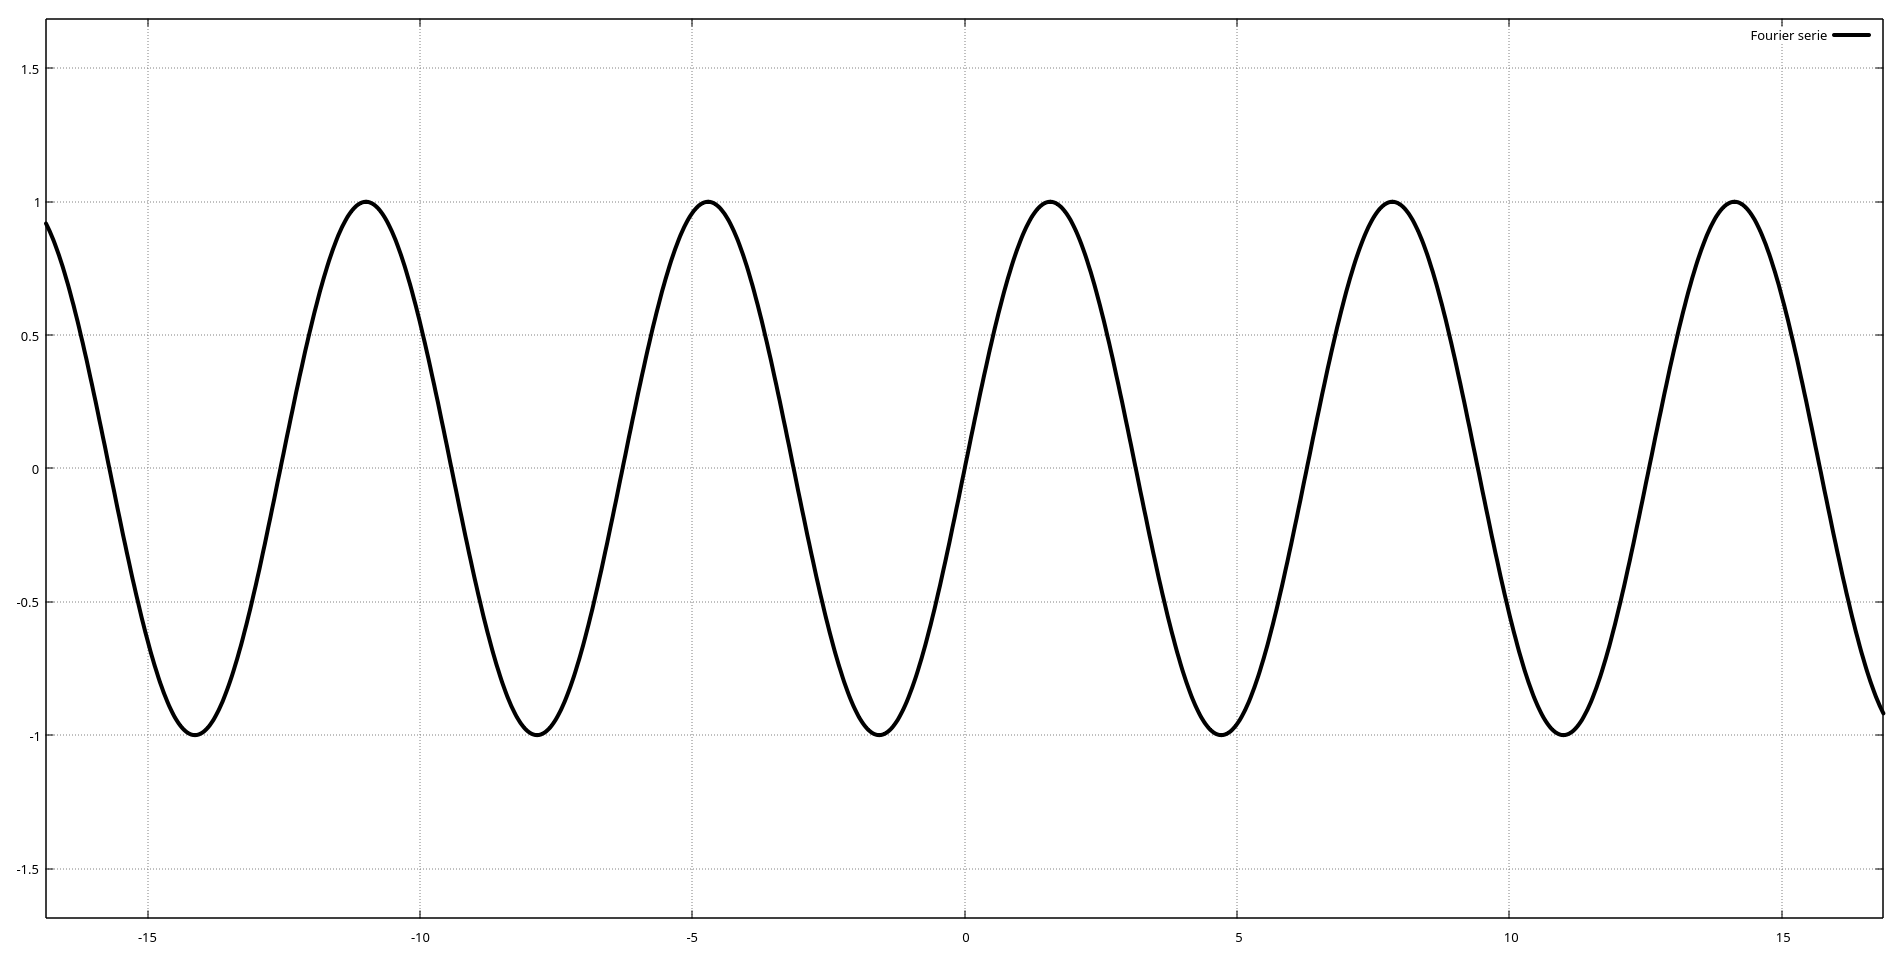
\includegraphics[width=\textwidth]{assets/gnuplot_sinx.png}
\caption*{
	\lr{\mintinline{bash}{fouriersolver 'sin(x)' -a '-M_PI' -b 'M_PI' -g}}
}
\end{figure}

حال تابع دیگری مانند
$x^3$
را با $n$ متفاوت و دقت‌های متفاوت بررسی خواهیم کرد.

\begin{figure}[H]
\subfigr{assets/gnuplot_x3_1.png}{\lr{N=1}}
\subfigr{assets/gnuplot_x3_2.png}{\lr{N=2}}
\\[\smallskipamount]
\subfigr{assets/gnuplot_x3_5.png}{\lr{N=5}}
\subfigr{assets/gnuplot_x3_20.png}{\lr{N=20}}
\\[\smallskipamount]
\subfigr{assets/gnuplot_x3_100.png}{\lr{N=100}}
\subfigr{assets/gnuplot_x3_500.png}{\lr{N=500}}

\caption*{
	\lr{\mintinline{bash}{fouriersolver 'pow(x, 3)' -a '-2' -b '2' -g -n N}}
}
\end{figure}

با بررسی خروجی‌ها در این گزارش در میابیم که به درستی سری فوریه ترسیم شده است. نکته ای که حائز اهمیت است
این می‌باشد که \lr{N} بیشت از ۱۰۰ در برنامه \lr{gnuplot} نه تنها خروجی بهتری ارائه نمی‌دهد، بلکه باعث بروز مشکلاتی می‌شود
که با تنظیمات بیشتری می‌توان آنها را بهبود یافت. اما درکل \lr{gnuplot} مشکلاتی دارد و دلیلی وجود ندارد که \lr{N} را بیش از ۱۰۰ گذاشت.
در ادامه این گزارش پلتفرم‌های دیگر رسم نمودار بررسی خواهند شد.

\subsubsection{ایجاد خروجی اسکی}
پارامتر \lr{-d} به \lr{gnuplot} می‌فهماند که باید خروجی را در ترمینال و به فرمت اسکی
\LTRfootnote{ASCII}
نمایش دهد.

\begin{figure}[H]
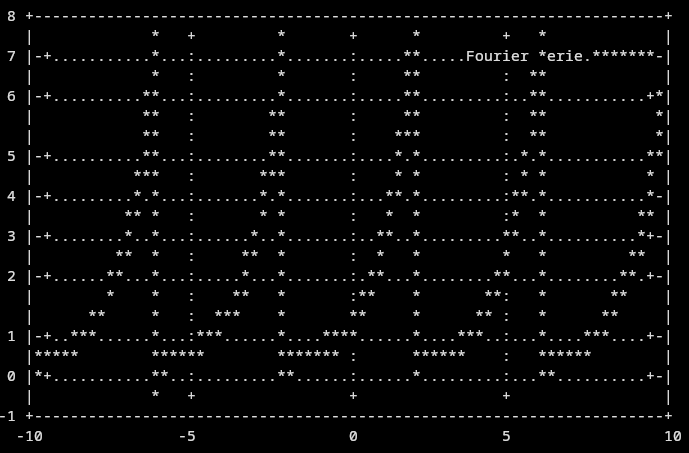
\includegraphics[width=\textwidth]{assets/gnuplot_term.png}
\caption*{
	\lr{\mintinline{bash}{fouriersolver "pow(M_E, x)" -a "-2" -b "2" -d}}
}
\end{figure}

\newpage
\subsubsection{تغییر نمونه‌ها}
\lr{gnuplot}
آپشنی دارد که با آن نمونه‌های خود را بیشتر می‌کند. در این حالت زمانی که تصویر را کوچک می‌کنید هماهنگی بیشتری خواهد داشت.
البته که برنامه \lr{gnuplot} همزمان با بیشتر شدن نمیونه‌ها کند تر نیز خواهد شد. در زیر تفاوت خروجی بر اساس تغییر نمونه ها
در شرایط یکسان دیده می‌شود. با بررسی خروجی‌ها بدیهیست که هرچه تعداد نمونه‌های \lr{gnuplot} بیشتر باشد، خروجی دقیق تر
و مطلوب تر خواهد بود.

\begin{figure}[H]
\subfigr{assets/gnuplot_coshx_s50.png}{\lr{S=50}}
\subfigr{assets/gnuplot_coshx_s100.png}{\lr{S=100}}
\\[\smallskipamount]
\subfigr{assets/gnuplot_coshx_s1000.png}{\lr{S=1000}}
\subfigr{assets/gnuplot_coshx_s2000.png}{\lr{S=2000}}
\\[\smallskipamount]
\subfigr{assets/gnuplot_coshx_s5000.png}{\lr{S=5000}}
\subfigr{assets/gnuplot_coshx_s10000.png}{\lr{S=10000}}

\caption*{
	\lr{\mintinline{bash}{fouriersolver 'cosh(x)' -a '-2' -b '2' -g -n 100 -g -s S}}
}
\end{figure}

\subsubsection{نمایش عبارات}
این آپشن صرفا آنچه به \lr{gnuplot} ارسال می‌شود را نمایش می‌دهد و با فلگ \lr{-f} فعال می‌شود.

\begin{latin}
\begin{minted}{bash}
$ ./fouriersolver 'sqrt(x)' -a '-2' -b '2' -g -n 5 -f
+-nan*cos(x*0*pi/2.000000)+-nan*sin(x*0*pi/2.000000)+-nan*cos(x*1*pi/2.000000)+-nan*sin(x*1*pi/2.000000)+-nan*cos(x*2*pi/2.000000)+-nan*sin(x*2*pi/2.000000)+-nan*cos(x*3*pi/2.000000)+-nan*sin(x*3*pi/2.000000)+-nan*cos(x*4*pi/2.000000)+-nan*sin(x*4*pi/2.000000)+-nan*cos(x*5*pi/2.000000)+-nan*sin(x*5*pi/2.000000)
$
\end{minted}
\end{latin}

\newpage
\subsection{\lr{desmos}}
یکپارچه سازی با دو پلتفرم آنلاین دیگر به این صورت است که خروجی حاصل را باید در کلیپ‌برد ذخیره کنید و آنرا در وبسایت کپی کنید.
برای دریافت خروجی سازگار با \lr{desmos} از پارامتر \lr{-m} می‌توانید استفاده کنید.
در سیستم‌های یونیکسی که از \lr{X11} استفاده می‌کنند می‌توانید از \lr{xclip} استفاده کنید و خروجی را مستقیم کپی کنید.
برای بررسی خروجی این اپلیکیشن از همان ورودی‌هایی که در \lr{gnuplot} وارد کرده بودیم استفاده می‌کنیم.

در \lr{desmos} نیز بیش از $N=100$ بهتر است ورودی ندهید. بر اساس گزارش خروجی زیر، در میابیم که این ابزار نیز محدودیت‌هایی دارد
و در صورتی که بیش آز آنچه طراحانش پیش‌بینی کردند ورودی دریافت کند به مشکل بر خواهد خورد. در اینجا تعداد نمونه‌ها را خود ابزار
تنظیم می‌کند. درضمن در حالتی که \lr{N} برابر ۲۵۰ است، وب اپلیکیشن نمی‌تواند به درستی کار کند و ممکن است تب مرورگر شما بسته شود.
علت آن پردازش بیش از اندازه می‌باشد. نمی‌توانید بیش از آنچه باید در این اپلیکیشن تحت وب پردازش انجام دهید.

\begin{figure}[H]
\subfigr{assets/desmos_x3_1.png}{\lr{N=1}}
\subfigr{assets/desmos_x3_2.png}{\lr{N=2}}
\\[\smallskipamount]
\subfigr{assets/desmos_x3_5.png}{\lr{N=5}}
\subfigr{assets/desmos_x3_20.png}{\lr{N=20}}
\\[\smallskipamount]
\subfigr{assets/desmos_x3_100.png}{\lr{N=100}}
\subfigr{assets/desmos_x3_250.png}{\lr{N=250}}

\caption*{
	\lr{\mintinline{bash}{fouriersolver 'pow(x, 3)' -a '-2' -b '2' -m -n N | xclip -selection clipboard}}
}
\end{figure}

\newpage
\subsection{\lr{geogebra}}
عملکرد یکپارچه‌سازی پروژه با \lr{geogebra} دقیقا مشابه \lr{desmos} در قسمت قبل می‌باشد. با این تفاوت که فلگ لازم برای
تولید خروجی مورد نیاز برای \lr{geogebra}،‌ \lr{-r} می‌باشد. با تجربه ای اندک متوجه می‌شوید که ذاتا این پلتفرم سرعت لود کمتری
به نسبت \lr{desmos} دارد. میزان مصرف رم و سی‌پیو این اپلیکیشن بسیار بالا بوده و مقدار \lr{N} حتی در ۱۰۰ هم مشکل‌ساز است.
حتی برای مقدار ۱۰ هم چندین ثانیه طول می‌کشد تا سری ترسیم شود.

\begin{figure}[H]
\subfigr{assets/geogebra_x3_1.png}{\lr{N=1}}
\subfigr{assets/geogebra_x3_2.png}{\lr{N=2}}
\\[\smallskipamount]
\subfigr{assets/geogebra_x3_5.png}{\lr{N=5}}
\subfigr{assets/geogebra_x3_20.png}{\lr{N=20}}
\\[\smallskipamount]
\subfigr{assets/geogebra_x3_50.png}{\lr{N=50}}
\subfigr{assets/geogebra_x3_100.png}{\lr{N=100}}

\caption*{
	\lr{\mintinline{bash}{fouriersolver 'pow(x, 3)' -a '-2' -b '2' -r -n N | xclip -selection clipboard}}
}
\end{figure}

\subsection{مقایسه بک‌اندهای مختلف ترسیم سری}
با مقایسه هر سه بک‌اند مذکور در ابتدا در میابیم که طراحی موجود به ازای
$N>100$
ناکارآمد خواهد بود. اگر بخواهیم سهولت استفاده، نزدیک بودن خروجی به واقعیت، سرعت و قابلیت تنظیم را درنظر بگیریم
گزینه \lr{gnuplot} از موارد دیگر بهتر عمل می‌کند و می‌تواند مورد استفاده قراره گرفته شود.
برای بررسی ارتباط سرعت اجرای برنامه و مقدار \lr{N} باید این نکته را اشاره کرد که به دلیل محدودیت مذکور، برای مقادیر کمتر از ۱۰۰
تفاوت چندانی وجود ندارد. لزا نیازی به بررسی نیست.

\newpage
\subsection{تاثیر دقت محاسبه انتگرال در رسم سری}
با بررسی خروجی‌ها در دقت‌های متفاوت می‌توان استنتاج کرد دقت بیش از مقدار پیشفرض تنها باعث کند شدن برنامه می‌شود
و ناکارآمد می‌باشد. محاسبه انتگرال معین بواسطه الگوریتم‌هایی که برای زبان‌های برنامه‌نویسی ارائه شده اند جواب دقیق را نخواهد یافت.
تنها با دقت خاصی می‌تواند انتگرال معین را محاسبه کند. در عمل نیز دقت بیش از پیشفرض کارآمد نخواهد بود.

\begin{figure}[H]
\subfigr{assets/gnuplot_x2_100_p0.png}{\lr{P=1}}
\subfigr{assets/gnuplot_x2_100_p1.png}{\lr{P=0.1}}
\\[\smallskipamount]
\subfigr{assets/gnuplot_x2_100_p2.png}{\lr{P=0.01}}
\subfigr{assets/gnuplot_x2_100_p3.png}{\lr{P=0.001}}
\\[\smallskipamount]
\subfigr{assets/gnuplot_x2_100_p4.png}{\lr{P=0.0001}}
\subfigr{assets/gnuplot_x2_100_p5.png}{\lr{P=0.00001}}

\caption*{
	\lr{\mintinline{bash}{fouriersolver 'pow(x, 2)' -a '-2' -b '2' -g -n 100  -s 10000 -p P}}
}
\end{figure}

\newpage
\section{مثال‌های متنوع رسم سری با \lr{gnuplot}}

\begin{figure}[H]
\subfigr{assets/sx.png}{$x$}
\subfigr{assets/sx2.png}{$x^2$}
\\[\smallskipamount]
\subfigr{assets/sx3.png}{$x^3$}
\subfigr{assets/sx4.png}{$x^4$}
\\[\smallskipamount]
\subfigr{assets/sex.png}{$e^x$}
\subfigr{assets/xpi.png}{$\frac{x}{\pi}$}
\end{figure}

\begin{figure}[H]
\subfigr{assets/sinx.png}{$\sin(x) in -\pi < x < \pi$}
\subfigr{assets/cosx.png}{$\cos(x) in -\pi < x < \pi$}
\\[\smallskipamount]
\subfigr{assets/sinh.png}{$\sinh(x)$}
\subfigr{assets/cosh.png}{$\cosh(x)$}
\\[\smallskipamount]
\subfigr{assets/abs.png}{$|x|$}
\subfigr{assets/floor.png}{$floor(x)$}
\end{figure}

\newpage
\section{عملکرد کد}
\subsection{عملکرد دریافت ورودی‌ها}
چالش‌برانگیز ترین بخش این پروژه دریافت یک عبارت ریاضی از کاربر بود. یکی از گزینه‌های روی میز استفاده از کتابخوانه‌های آماده ای
مانند \lr{muParser} بود. اما هدف این پروژه آموزشی می‌باشد و به همین دلیل حل این مسئله خود جذابیت کار می‌باشد.

سه ورودی $f(x)$ و بازه $x$ از سینتکس سی پیروی می‌کنند. طراحی این بخش نرم‌افزار اینگونه است که موقع هندل کردن ارگومان‌ها
تابع \lr{generate\_exp\_sharedlib} اجرا می‌شود. این تابع صرفا کدهای ورودی برنامه‌را داخل کد دیگری تذریق می‌کند و آن را به‌عنوان
فایل سی روی استوریج ذخیره می‌کند. این فایل حاوی سه تابع با نام‌های \lr{f, lowerl, upperl} بوده که \lr{l} به‌معنای حد یا \lr{limit} است.
پس از آن همین فایل ایجاد شده کامپایل شده و از آن یک کتابخانه داینامیک
\LTRfootnote{Dynamic Library, Shared Library, so file}
با پسوند \lr{so} تولید می‌شود. کتابخانه‌های داینامیک مانند \lr{DLL} ها در ویندوز هستند اما در سیستم‌های یونیکسی.
پس از آن در \lr{main} همین کتابخانه داینامیک لود شده و ۳ تابع مذکور در \lr{callback} هایی از پیش تعریف شده لود می‌شوند.
درواقع مکانیزمی تعبیه کرده ایم که از بیرون برنامه به آن کد تذریق کنیم.

\begin{latin}
\begin{minted}{c}
int generate_exp_sharedlib(char *math_exp)
{
        FILE *f;

        if (!(f = fopen("/tmp/exp.c", "w")))
                return (EXIT_FAILURE);

        fprintf(f,
                "/* Generated by fourier.sh */\n"
                "#include <math.h>\n"
                "#include <stdlib.h>\n"
                "\n"
                "double f(double x)\n"
                "{\n"
                "        return %s;\n"
                "}\n"
                "\n"
                "double lowerl()\n"
                "{\n"
                "         return %s;\n"
                "}\n"
                "\n"
                "double upperl()\n"
                "{\n"
                "         return %s;\n"
                "}\n",
                math_exp, lowerl, upperl
               );
        fclose(f);

        system("cc -lm -shared -fPIC /tmp/exp.c -o /tmp/exp.so");
        flib_path = "/tmp/exp.so";
        return (EXIT_SUCCESS);
}
\end{minted}
\end{latin}

\subsection{محاسبه ضرایب فوریه}
بالاتر به الگوریتم محاسبه انتگرال اشاره شد. به‌سادگی پس از آن از فرمول فوریه برای محاسبه ضرایب فوریه استفاد همی‌کنیم.

\section{سخن نهایی}
پروژه ترسیم سری فوریه بسیار پروژه لذت‌بخش و سرگرم کننده ای برای من بود و گذر زمان را حتی در نوشتن گزارش آن حس نکردم.
کمالگرایی اجازه نداد که ساعات کمی را به این پروژه اختصاص بدم و دلتنگی زیاد برای توسعه نرم افزار سبب شد نسبتا زمان زیادی برای
این کار صرف کنم. هرچند این پروژه آنقدر دیده نخواهد شد اما یادآور دورانی از زندگی من است. مفاهیمی که در این پروژه استفاده شده است
شاید حاصل هزاران صفحه مطالعه فنی در حوزه مهندسی نرم‌افزار می‌باشد. مطالبی که پس از ماه‌ها دوری از این حوزه هنوز در ذهنم باقی مانده بودند.
خوشحالم که این پروژه بهم یادآوری کرد که منطق زیبای یونیکس و ساختارهای آن یک بار نیاز به یادگیری دارد.
جوزف فوریه در ابتدا سری فوریه را برای حل مسائل فیزیکی مانند ارتعاش ریسمان و انتقال گرما در دیسک رسانا ابداع کرد.
و من این پروژه را به جهت زیبا تر دیدن جهان و لذت‌جویی از این دنیای فانی توسعه دادم. کلیت محاسبه سری فوریه با زبانی مانند متلب
شاید با چند ساعت مطالعه قابل پیاده سازی بود. اما هدف غایی من از توسعه این سیستم صرف ۲ نمره نبود. همانطور که معتقد هستم
ارزش این کار بسیار فراتر از یک درس ۳ واحدی می‌باشد. این پروژه تمام شوق و ذوق من است که به‌واسطه دانش محدودی که دارم
در این ساعت در جهان ما چشم گشوده است. امیدوارم تک تک کسانی که این پاراگراف را مطالعه می‌کنند روزی به اندازه من از خلق و طراحی
یک ایده لذت ببرند.

باتشکر، علیرضا ارزه گر.

\end{document}

